\documentclass[twoside]{book}

% Packages required by doxygen
\usepackage{fixltx2e}
\usepackage{calc}
\usepackage{doxygen}
\usepackage[export]{adjustbox} % also loads graphicx
\usepackage{graphicx}
\usepackage[utf8]{inputenc}
\usepackage{makeidx}
\usepackage{multicol}
\usepackage{multirow}
\PassOptionsToPackage{warn}{textcomp}
\usepackage{textcomp}
\usepackage[nointegrals]{wasysym}
\usepackage[table]{xcolor}

% Font selection
\usepackage[T1]{fontenc}
\usepackage[scaled=.90]{helvet}
\usepackage{courier}
\usepackage{amssymb}
\usepackage{sectsty}
\renewcommand{\familydefault}{\sfdefault}
\allsectionsfont{%
  \fontseries{bc}\selectfont%
  \color{darkgray}%
}
\renewcommand{\DoxyLabelFont}{%
  \fontseries{bc}\selectfont%
  \color{darkgray}%
}
\newcommand{\+}{\discretionary{\mbox{\scriptsize$\hookleftarrow$}}{}{}}

% Page & text layout
\usepackage{geometry}
\geometry{%
  a4paper,%
  top=2.5cm,%
  bottom=2.5cm,%
  left=2.5cm,%
  right=2.5cm%
}
\tolerance=750
\hfuzz=15pt
\hbadness=750
\setlength{\emergencystretch}{15pt}
\setlength{\parindent}{0cm}
\setlength{\parskip}{3ex plus 2ex minus 2ex}
\makeatletter
\renewcommand{\paragraph}{%
  \@startsection{paragraph}{4}{0ex}{-1.0ex}{1.0ex}{%
    \normalfont\normalsize\bfseries\SS@parafont%
  }%
}
\renewcommand{\subparagraph}{%
  \@startsection{subparagraph}{5}{0ex}{-1.0ex}{1.0ex}{%
    \normalfont\normalsize\bfseries\SS@subparafont%
  }%
}
\makeatother

% Headers & footers
\usepackage{fancyhdr}
\pagestyle{fancyplain}
\fancyhead[LE]{\fancyplain{}{\bfseries\thepage}}
\fancyhead[CE]{\fancyplain{}{}}
\fancyhead[RE]{\fancyplain{}{\bfseries\leftmark}}
\fancyhead[LO]{\fancyplain{}{\bfseries\rightmark}}
\fancyhead[CO]{\fancyplain{}{}}
\fancyhead[RO]{\fancyplain{}{\bfseries\thepage}}
\fancyfoot[LE]{\fancyplain{}{}}
\fancyfoot[CE]{\fancyplain{}{}}
\fancyfoot[RE]{\fancyplain{}{\bfseries\scriptsize Generated by Doxygen }}
\fancyfoot[LO]{\fancyplain{}{\bfseries\scriptsize Generated by Doxygen }}
\fancyfoot[CO]{\fancyplain{}{}}
\fancyfoot[RO]{\fancyplain{}{}}
\renewcommand{\footrulewidth}{0.4pt}
\renewcommand{\chaptermark}[1]{%
  \markboth{#1}{}%
}
\renewcommand{\sectionmark}[1]{%
  \markright{\thesection\ #1}%
}

% Indices & bibliography
\usepackage{natbib}
\usepackage[titles]{tocloft}
\setcounter{tocdepth}{3}
\setcounter{secnumdepth}{5}
\makeindex

% Hyperlinks (required, but should be loaded last)
\usepackage{ifpdf}
\ifpdf
  \usepackage[pdftex,pagebackref=true]{hyperref}
\else
  \usepackage[ps2pdf,pagebackref=true]{hyperref}
\fi
\hypersetup{%
  colorlinks=true,%
  linkcolor=blue,%
  citecolor=blue,%
  unicode%
}

% Custom commands
\newcommand{\clearemptydoublepage}{%
  \newpage{\pagestyle{empty}\cleardoublepage}%
}

\usepackage{caption}
\captionsetup{labelsep=space,justification=centering,font={bf},singlelinecheck=off,skip=4pt,position=top}

%===== C O N T E N T S =====

\begin{document}

% Titlepage & ToC
\hypersetup{pageanchor=false,
             bookmarksnumbered=true,
             pdfencoding=unicode
            }
\pagenumbering{alph}
\begin{titlepage}
\vspace*{7cm}
\begin{center}%
{\Large My Project }\\
\vspace*{1cm}
{\large Generated by Doxygen 1.8.13}\\
\end{center}
\end{titlepage}
\clearemptydoublepage
\pagenumbering{roman}
\tableofcontents
\clearemptydoublepage
\pagenumbering{arabic}
\hypersetup{pageanchor=true}

%--- Begin generated contents ---
\chapter{Hierarchical Index}
\section{Class Hierarchy}
This inheritance list is sorted roughly, but not completely, alphabetically\+:\begin{DoxyCompactList}
\item \contentsline{section}{custom\+Draw}{\pageref{classcustom_draw}}{}
\item \contentsline{section}{extended\+Frame}{\pageref{classextended_frame}}{}
\item \contentsline{section}{Frame\+Queue}{\pageref{class_frame_queue}}{}
\item Key\+Point\begin{DoxyCompactList}
\item \contentsline{section}{custom\+Keypoint}{\pageref{classcustom_keypoint}}{}
\end{DoxyCompactList}
\end{DoxyCompactList}

\chapter{Class Index}
\section{Class List}
Here are the classes, structs, unions and interfaces with brief descriptions\+:\begin{DoxyCompactList}
\item\contentsline{section}{\hyperlink{classcustom_draw}{custom\+Draw} }{\pageref{classcustom_draw}}{}
\item\contentsline{section}{\hyperlink{classcustom_keypoint}{custom\+Keypoint} }{\pageref{classcustom_keypoint}}{}
\item\contentsline{section}{\hyperlink{classextended_frame}{extended\+Frame} \\*The \hyperlink{classextended_frame}{extended\+Frame} class }{\pageref{classextended_frame}}{}
\item\contentsline{section}{\hyperlink{class_frame_queue}{Frame\+Queue} \\*The \hyperlink{class_frame_queue}{Frame\+Queue} class }{\pageref{class_frame_queue}}{}
\end{DoxyCompactList}

\chapter{Class Documentation}
\hypertarget{classcustom_draw}{}\section{custom\+Draw Class Reference}
\label{classcustom_draw}\index{custom\+Draw@{custom\+Draw}}
\subsection*{Static Public Member Functions}
\begin{DoxyCompactItemize}
\item 
static int \hyperlink{classcustom_draw_aced241b508544a5dea840f97fe1f2e2c}{draw\+Keypoint\+Circle} (Mat \&image, Key\+Point \&Kpoint, Scalar color)
\begin{DoxyCompactList}\small\item\em draw\+Keypoint\+Circle Отрисовывает окружность с центром в точке, соответствующей координатам переданной особой точки. \end{DoxyCompactList}\item 
static int \hyperlink{classcustom_draw_ab2d07b0922ada8467a5eadf5c26fc7b7}{draw\+Keypoint\+Xmark} (Mat \&image, Key\+Point \&Kpoint, Scalar color)
\begin{DoxyCompactList}\small\item\em draw\+Keypoint\+Xmark Отрисовывает X-\/метку с центром в точке, соответствующей координатам переданной особой точки. \end{DoxyCompactList}\item 
static int \hyperlink{classcustom_draw_a5bcac7ca4e055881b17d36b9c70ead92}{draw\+Line\+Between\+Keypoints} (Mat \&image, Key\+Point \&Kpoint1, Key\+Point \&Kpoint2, Scalar color)
\begin{DoxyCompactList}\small\item\em draw\+Line\+Between\+Keypoints Рисует линию между двумя заданными особыми точками \end{DoxyCompactList}\item 
static Scalar \hyperlink{classcustom_draw_a9b316ec0c5b586ab78d734c121e584c5}{create\+Color} (uint32\+\_\+t color)
\begin{DoxyCompactList}\small\item\em create\+Color Генерирует цвет по названию из таблицы цветов в \hyperlink{colors_8hpp_source}{colors.\+hpp} \end{DoxyCompactList}\item 
static int \hyperlink{classcustom_draw_af350b300142db4bfe210b57a40e7a610}{draw\+Matches} (Mat \&image, vector$<$ Key\+Point $>$ kps1, vector$<$ Key\+Point $>$ kps2, vector$<$ D\+Match $>$ matches, Scalar color)
\begin{DoxyCompactList}\small\item\em draw\+Matches Рисует линию между особыми точками \end{DoxyCompactList}\end{DoxyCompactItemize}


\subsection{Member Function Documentation}
\mbox{\Hypertarget{classcustom_draw_a9b316ec0c5b586ab78d734c121e584c5}\label{classcustom_draw_a9b316ec0c5b586ab78d734c121e584c5}} 
\index{custom\+Draw@{custom\+Draw}!create\+Color@{create\+Color}}
\index{create\+Color@{create\+Color}!custom\+Draw@{custom\+Draw}}
\subsubsection{\texorpdfstring{create\+Color()}{createColor()}}
{\footnotesize\ttfamily Scalar custom\+Draw\+::create\+Color (\begin{DoxyParamCaption}\item[{uint32\+\_\+t}]{color }\end{DoxyParamCaption})\hspace{0.3cm}{\ttfamily [static]}}



create\+Color Генерирует цвет по названию из таблицы цветов в \hyperlink{colors_8hpp_source}{colors.\+hpp} 


\begin{DoxyParams}{Parameters}
{\em color} & \\
\hline
\end{DoxyParams}
\begin{DoxyReturn}{Returns}

\end{DoxyReturn}
\mbox{\Hypertarget{classcustom_draw_aced241b508544a5dea840f97fe1f2e2c}\label{classcustom_draw_aced241b508544a5dea840f97fe1f2e2c}} 
\index{custom\+Draw@{custom\+Draw}!draw\+Keypoint\+Circle@{draw\+Keypoint\+Circle}}
\index{draw\+Keypoint\+Circle@{draw\+Keypoint\+Circle}!custom\+Draw@{custom\+Draw}}
\subsubsection{\texorpdfstring{draw\+Keypoint\+Circle()}{drawKeypointCircle()}}
{\footnotesize\ttfamily int custom\+Draw\+::draw\+Keypoint\+Circle (\begin{DoxyParamCaption}\item[{Mat \&}]{image,  }\item[{Key\+Point \&}]{Kpoint,  }\item[{Scalar}]{color }\end{DoxyParamCaption})\hspace{0.3cm}{\ttfamily [static]}}



draw\+Keypoint\+Circle Отрисовывает окружность с центром в точке, соответствующей координатам переданной особой точки. 


\begin{DoxyParams}{Parameters}
{\em image\mbox{[}in\mbox{]}} & \\
\hline
{\em Kpoint\mbox{[}in\mbox{]}} & \\
\hline
{\em color\mbox{[}in\mbox{]}} & \\
\hline
\end{DoxyParams}
\begin{DoxyReturn}{Returns}

\end{DoxyReturn}
\mbox{\Hypertarget{classcustom_draw_ab2d07b0922ada8467a5eadf5c26fc7b7}\label{classcustom_draw_ab2d07b0922ada8467a5eadf5c26fc7b7}} 
\index{custom\+Draw@{custom\+Draw}!draw\+Keypoint\+Xmark@{draw\+Keypoint\+Xmark}}
\index{draw\+Keypoint\+Xmark@{draw\+Keypoint\+Xmark}!custom\+Draw@{custom\+Draw}}
\subsubsection{\texorpdfstring{draw\+Keypoint\+Xmark()}{drawKeypointXmark()}}
{\footnotesize\ttfamily int custom\+Draw\+::draw\+Keypoint\+Xmark (\begin{DoxyParamCaption}\item[{Mat \&}]{image,  }\item[{Key\+Point \&}]{Kpoint,  }\item[{Scalar}]{color }\end{DoxyParamCaption})\hspace{0.3cm}{\ttfamily [static]}}



draw\+Keypoint\+Xmark Отрисовывает X-\/метку с центром в точке, соответствующей координатам переданной особой точки. 


\begin{DoxyParams}{Parameters}
{\em image} & \\
\hline
{\em Kpoint} & \\
\hline
{\em color} & \\
\hline
\end{DoxyParams}
\begin{DoxyReturn}{Returns}

\end{DoxyReturn}
\begin{DoxyWarning}{Warning}
не реализован 
\end{DoxyWarning}
\mbox{\Hypertarget{classcustom_draw_a5bcac7ca4e055881b17d36b9c70ead92}\label{classcustom_draw_a5bcac7ca4e055881b17d36b9c70ead92}} 
\index{custom\+Draw@{custom\+Draw}!draw\+Line\+Between\+Keypoints@{draw\+Line\+Between\+Keypoints}}
\index{draw\+Line\+Between\+Keypoints@{draw\+Line\+Between\+Keypoints}!custom\+Draw@{custom\+Draw}}
\subsubsection{\texorpdfstring{draw\+Line\+Between\+Keypoints()}{drawLineBetweenKeypoints()}}
{\footnotesize\ttfamily int custom\+Draw\+::draw\+Line\+Between\+Keypoints (\begin{DoxyParamCaption}\item[{Mat \&}]{image,  }\item[{Key\+Point \&}]{Kpoint1,  }\item[{Key\+Point \&}]{Kpoint2,  }\item[{Scalar}]{color }\end{DoxyParamCaption})\hspace{0.3cm}{\ttfamily [static]}}



draw\+Line\+Between\+Keypoints Рисует линию между двумя заданными особыми точками 


\begin{DoxyParams}{Parameters}
{\em image} & \\
\hline
{\em Kpoint1} & \\
\hline
{\em Kpoint2} & \\
\hline
{\em color} & \\
\hline
\end{DoxyParams}
\begin{DoxyReturn}{Returns}

\end{DoxyReturn}
\begin{DoxyWarning}{Warning}
T\+O\+DO\+: добавить настройку отображения толщины и размера 
\end{DoxyWarning}
\mbox{\Hypertarget{classcustom_draw_af350b300142db4bfe210b57a40e7a610}\label{classcustom_draw_af350b300142db4bfe210b57a40e7a610}} 
\index{custom\+Draw@{custom\+Draw}!draw\+Matches@{draw\+Matches}}
\index{draw\+Matches@{draw\+Matches}!custom\+Draw@{custom\+Draw}}
\subsubsection{\texorpdfstring{draw\+Matches()}{drawMatches()}}
{\footnotesize\ttfamily int custom\+Draw\+::draw\+Matches (\begin{DoxyParamCaption}\item[{Mat \&}]{image,  }\item[{vector$<$ Key\+Point $>$}]{kps1,  }\item[{vector$<$ Key\+Point $>$}]{kps2,  }\item[{vector$<$ D\+Match $>$}]{matches,  }\item[{Scalar}]{color }\end{DoxyParamCaption})\hspace{0.3cm}{\ttfamily [static]}}



draw\+Matches Рисует линию между особыми точками 


\begin{DoxyParams}{Parameters}
{\em image} & \\
\hline
{\em kps1} & \\
\hline
{\em kps2} & \\
\hline
{\em matches} & \\
\hline
{\em color} & \\
\hline
\end{DoxyParams}
\begin{DoxyReturn}{Returns}

\end{DoxyReturn}


The documentation for this class was generated from the following files\+:\begin{DoxyCompactItemize}
\item 
custom\+\_\+drawing.\+hpp\item 
custom\+\_\+drawing.\+cpp\end{DoxyCompactItemize}

\hypertarget{classcustom_keypoint}{}\section{custom\+Keypoint Class Reference}
\label{classcustom_keypoint}\index{custom\+Keypoint@{custom\+Keypoint}}
Inheritance diagram for custom\+Keypoint\+:\begin{figure}[H]
\begin{center}
\leavevmode
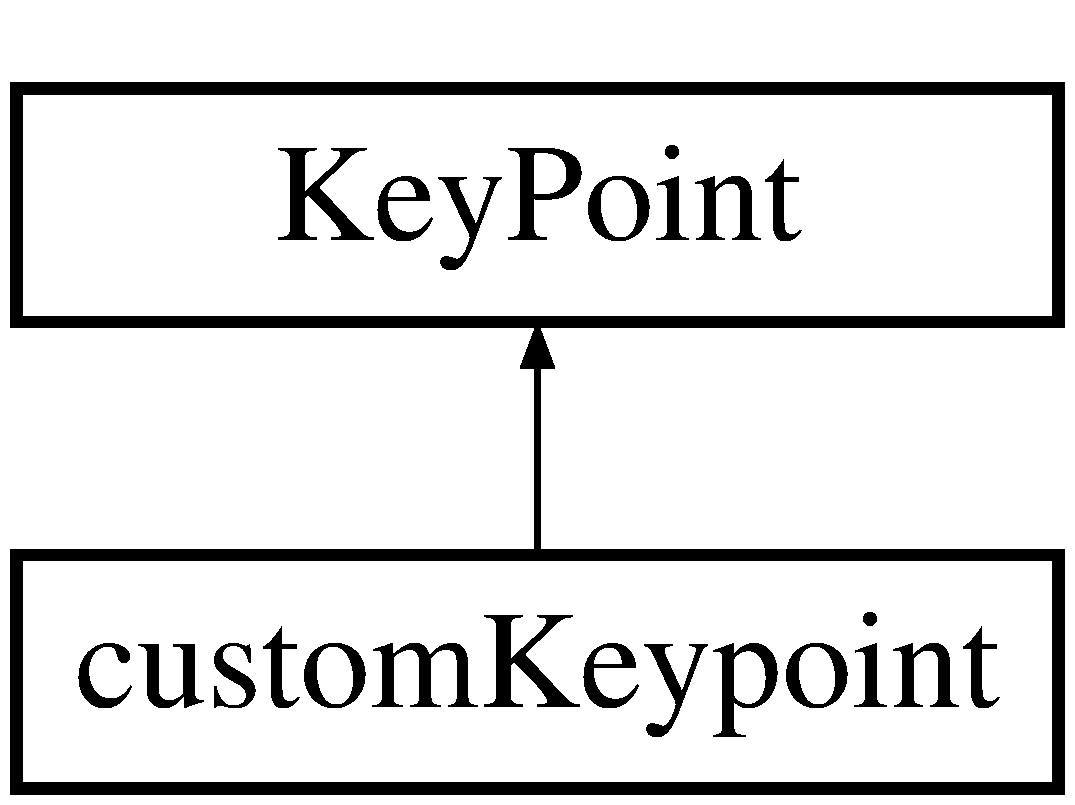
\includegraphics[height=2.000000cm]{classcustom_keypoint}
\end{center}
\end{figure}


The documentation for this class was generated from the following files\+:\begin{DoxyCompactItemize}
\item 
customkeypoint.\+h\item 
customkeypoint.\+cpp\end{DoxyCompactItemize}

\hypertarget{classextended_frame}{}\section{extended\+Frame Class Reference}
\label{classextended_frame}\index{extended\+Frame@{extended\+Frame}}


The \hyperlink{classextended_frame}{extended\+Frame} class.  




{\ttfamily \#include $<$extendedframe.\+h$>$}

\subsection*{Public Member Functions}
\begin{DoxyCompactItemize}
\item 
\hyperlink{classextended_frame_a22ce1e80c5583831eb81ac280c544136}{extended\+Frame} (Mat \&input\+\_\+frame, Ptr$<$ xfeatures2d\+::\+S\+U\+RF $>$ \&surf\+\_\+detector\+\_\+obj)
\begin{DoxyCompactList}\small\item\em \hyperlink{classextended_frame}{extended\+Frame} Конструктор \end{DoxyCompactList}\item 
\mbox{\Hypertarget{classextended_frame_a153ceb6cb957d38900f172c6ab11091c}\label{classextended_frame_a153ceb6cb957d38900f172c6ab11091c}} 
const Mat \& {\bfseries get\+Frame} ()
\item 
\mbox{\Hypertarget{classextended_frame_a795d9683335223e7d5e699f36d500e32}\label{classextended_frame_a795d9683335223e7d5e699f36d500e32}} 
const Mat \& {\bfseries get\+Descriptors} ()
\item 
\mbox{\Hypertarget{classextended_frame_a15f7d722562941cbcd672aa96153ae44}\label{classextended_frame_a15f7d722562941cbcd672aa96153ae44}} 
const vector$<$ Key\+Point $>$ \& {\bfseries get\+Keypoint\+Vector} ()
\end{DoxyCompactItemize}
\subsection*{Public Attributes}
\begin{DoxyCompactItemize}
\item 
\mbox{\Hypertarget{classextended_frame_ae2e741f3d4423653ce0f02caae6cce39}\label{classextended_frame_ae2e741f3d4423653ce0f02caae6cce39}} 
Mat \hyperlink{classextended_frame_ae2e741f3d4423653ce0f02caae6cce39}{frame}
\begin{DoxyCompactList}\small\item\em frame Исходное изображение \end{DoxyCompactList}\item 
\mbox{\Hypertarget{classextended_frame_a2db09e4d1897e028982017f83270c355}\label{classextended_frame_a2db09e4d1897e028982017f83270c355}} 
vector$<$ Key\+Point $>$ \hyperlink{classextended_frame_a2db09e4d1897e028982017f83270c355}{frame\+\_\+keypoints}
\begin{DoxyCompactList}\small\item\em frame\+\_\+keypoints Вектор особых точек текущего кадра \end{DoxyCompactList}\item 
\mbox{\Hypertarget{classextended_frame_a01d160021a186399a58af49c0cd4c97f}\label{classextended_frame_a01d160021a186399a58af49c0cd4c97f}} 
Mat \hyperlink{classextended_frame_a01d160021a186399a58af49c0cd4c97f}{frame\+\_\+descriptors}
\begin{DoxyCompactList}\small\item\em frame\+\_\+descriptors Дескрипторы особых точек текущего кадра \end{DoxyCompactList}\end{DoxyCompactItemize}


\subsection{Detailed Description}
The \hyperlink{classextended_frame}{extended\+Frame} class. 

Класс \char`\"{}расширенного\char`\"{} кадра, содержащего как само изображение, так и особые точки с дескрипторами 

\subsection{Constructor \& Destructor Documentation}
\mbox{\Hypertarget{classextended_frame_a22ce1e80c5583831eb81ac280c544136}\label{classextended_frame_a22ce1e80c5583831eb81ac280c544136}} 
\index{extended\+Frame@{extended\+Frame}!extended\+Frame@{extended\+Frame}}
\index{extended\+Frame@{extended\+Frame}!extended\+Frame@{extended\+Frame}}
\subsubsection{\texorpdfstring{extended\+Frame()}{extendedFrame()}}
{\footnotesize\ttfamily extended\+Frame\+::extended\+Frame (\begin{DoxyParamCaption}\item[{Mat \&}]{input\+\_\+frame,  }\item[{Ptr$<$ xfeatures2d\+::\+S\+U\+RF $>$ \&}]{surf\+\_\+detector\+\_\+obj }\end{DoxyParamCaption})}



\hyperlink{classextended_frame}{extended\+Frame} Конструктор 


\begin{DoxyParams}[1]{Parameters}
\mbox{\tt in}  & {\em input\+\_\+frame} & Исходное изображение \\
\hline
\mbox{\tt in}  & {\em surf\+\_\+detector\+\_\+obj} & Ссылка на детектор \\
\hline
\end{DoxyParams}


The documentation for this class was generated from the following files\+:\begin{DoxyCompactItemize}
\item 
extendedframe.\+h\item 
extendedframe.\+cpp\end{DoxyCompactItemize}

\hypertarget{class_frame_queue}{}\section{Frame\+Queue Class Reference}
\label{class_frame_queue}\index{Frame\+Queue@{Frame\+Queue}}


The \hyperlink{class_frame_queue}{Frame\+Queue} class.  




{\ttfamily \#include $<$framequeue.\+h$>$}

\subsection*{Public Member Functions}
\begin{DoxyCompactItemize}
\item 
\mbox{\Hypertarget{class_frame_queue_ac21733d5447ae4d0e1d946d500434f4b}\label{class_frame_queue_ac21733d5447ae4d0e1d946d500434f4b}} 
{\bfseries Frame\+Queue} (Video\+Capture \&src, uint32\+\_\+t max\+\_\+frames)
\item 
\mbox{\Hypertarget{class_frame_queue_aab2fde0b8bee872c5db389d568928054}\label{class_frame_queue_aab2fde0b8bee872c5db389d568928054}} 
void {\bfseries move\+Queue} ()
\item 
\mbox{\Hypertarget{class_frame_queue_a5eee81a87da92160507101252079f43b}\label{class_frame_queue_a5eee81a87da92160507101252079f43b}} 
int {\bfseries set\+Max\+Frames} (uint32\+\_\+t num)
\end{DoxyCompactItemize}


\subsection{Detailed Description}
The \hyperlink{class_frame_queue}{Frame\+Queue} class. 

Класс, реализующий очередь расширенных кадров (\hyperlink{classextended_frame}{extended\+Frame}). 

The documentation for this class was generated from the following files\+:\begin{DoxyCompactItemize}
\item 
framequeue.\+h\item 
framequeue.\+cpp\end{DoxyCompactItemize}

%--- End generated contents ---

% Index
\backmatter
\newpage
\phantomsection
\clearemptydoublepage
\addcontentsline{toc}{chapter}{Index}
\printindex

\end{document}
